\section{Owsianka z owocami}
\bigskip
\small
\begin{minipage}{0.45\textwidth}
    \noindent \textbf{Czas:} 10 minut\\
    \textbf{Poziom trudności:} łatwy
\end{minipage}
\begin{minipage}{0.45\textwidth}
    \noindent \textbf{Ilość sprzątania:} minimalna\\
    \textbf{Wymagany mysi sprzęt:} -
\end{minipage}
\normalsize
\vspace{0.5cm}

\begin{multicols}{2}
\subsection*{Składniki}
\begin{itemize}
    \item 3 kopiaste łyżki błyskawicznych płatków owsianych
    \item 1 szklanka mleka
    \item 1 płaska łyżka miodu/cukru
    \item 1 łyżeczka nasionek chia (opcjonalnie)
    \item 1 łyżeczka siemienia lnianego (opcjonalnie)
\end{itemize}
\columnbreak
\begin{figure}[H]
    \centering
    \fbox{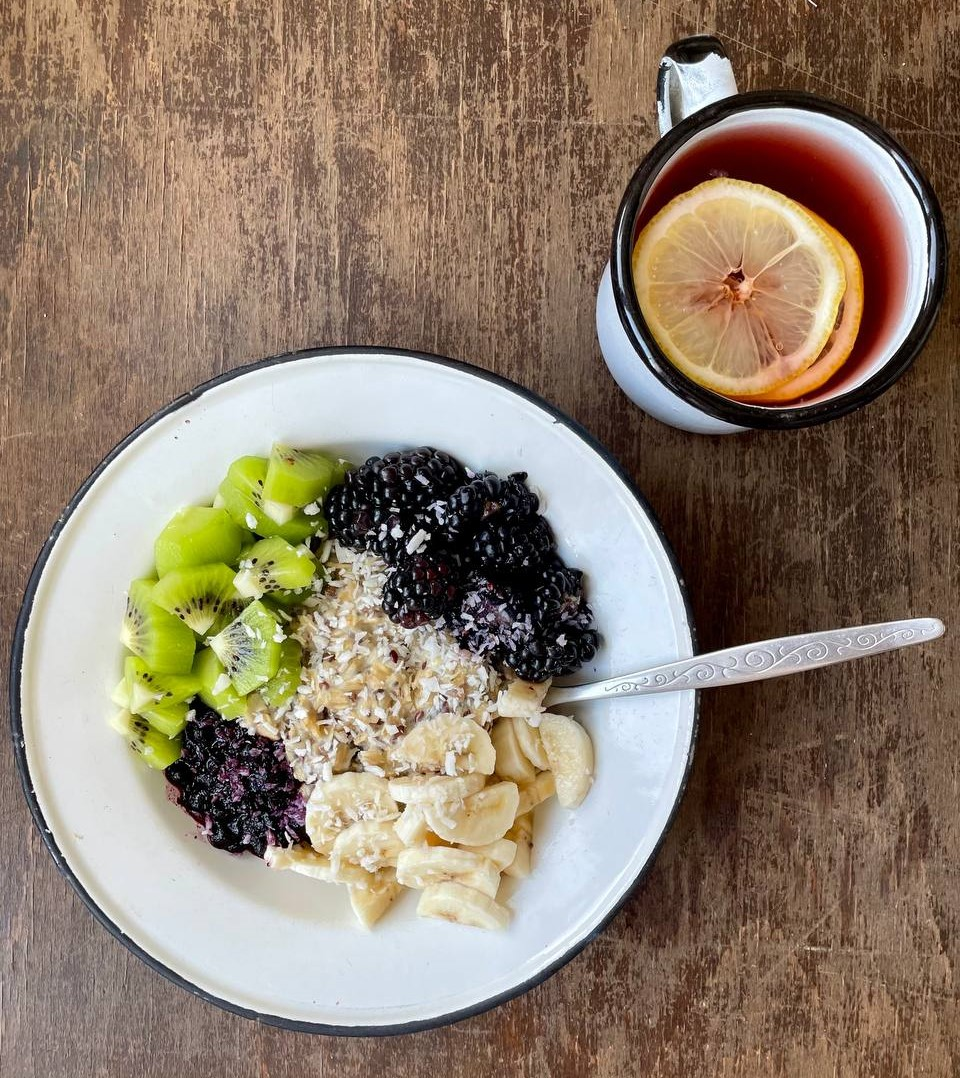
\includegraphics[width=0.35\textwidth]{images/owsianka.jpg}}
\end{figure}
\end{multicols}

\vspace{0.5cm}
\subsection*{Instruktaż}
\begin{enumerate}
    \item Płatki i nasiona wsypać do niewielkiego garnuszka, zalać mlekiem i mieszać od czasu do czasu aż mleko zacznie bulgotać.
    \item Gdy mleko osiągnie wysoką temperaturę, mieszać energicznie przez ok. 2 minuty.
\end{enumerate}

\vspace{0.5cm}
\small
\subsection*{Propozycja podania}
Z kawałkami czekolady, z jogurtem greckim, z owocami, z masłem orzechowym, z kremem czekoladowym, z wiórkami kokosowymi, z syropem klonowym.
\vspace{0.3cm}

\subsection*{Dodatkowe uwagi}
Owsiankę można urozmaicić smakowo poprzez dodanie do mleka cynamonu, przyprawy do piernika, kakao, masła orzechowego, płatków śniadaniowych, pokrojonego banana lub innych owoców, kawałków czekolady bądź orzechów.
\newpage